\documentclass[../main.tex]{subfiles}


\usepackage{nopageno} %Seitenzahlen auf richtiger Seite 

\usepackage[left=2cm, right=2cm, top=2cm, includehead, includefoot, headheight=17pt]{geometry}

\usepackage[utf8x]{inputenc}
\usepackage[english]{babel}
\usepackage{amsmath,amssymb,amsthm}
\usepackage{framed}
\usepackage{wasysym}
\usepackage[T1]{fontenc} %Silbentrennung 
\usepackage{color} %Farbe
\usepackage{graphicx}
\usepackage{float}%Grafik am gleichen Ort plazieren
%pdf. png. einfach eingliedern
\usepackage{subfigure} %Grafiken nebeneinander
\usepackage{pdfpages}
\usepackage{ulem} 	%\uuline{urgent}    % doppelt unterstreichen
%\uwave{boat}      % unterschlängeln
%\sout{wrong}       % durchstreichen
%\xout{removed}     % ausstreichen mit //////.

\usepackage{tikz}
\usetikzlibrary{trees}
\usetikzlibrary{plotmarks}
\usetikzlibrary{angles,quotes,babel}
\usetikzlibrary{shadings}
\usetikzlibrary{patterns}
\usetikzlibrary{matrix}
\usetikzlibrary{arrows}
\usetikzlibrary{calc}

\usepackage{pgfplots}
\usepackage{pgf-pie}
\pgfplotsset{compat=1.10}
\usepgfplotslibrary{statistics}
\usepgfplotslibrary{fillbetween}

\usepackage{tkz-euclide}
\usepackage{enumerate}
\usepackage{stmaryrd}
\usepackage{tabularx}
\usepackage{wrapfig}
\usepackage{epsdice}
\usepackage{multirow}
\usepackage{rotating}
\usepackage{pdflscape}
\usepackage{fancyhdr}

\pagestyle{fancy} %eigener Seitenstil
\fancyhf{} %alle Kopf- und Fußzeilenfelder bereinigen
\fancyhead[L]{} %Kopfzeile links
\fancyhead[C]{} %zentrierte Kopfzeile
\fancyhead[R]{} %Kopfzeile rechts
\renewcommand{\headrulewidth}{0.4pt} %obere Trennlinie
\fancyfoot[C]{\thepage} %Seitennummer
\renewcommand{\footrulewidth}{0.4pt} %untere Trennlinie

% Number spaces 
\newcommand{\CC}{\ensuremath{\mathbb{C}}}
\newcommand{\RR}{\ensuremath{\mathbb{R}}}
\newcommand{\QQ}{\ensuremath{\mathbb{Q}}}
\newcommand{\ZZ}{\ensuremath{\mathbb{Z}}}
\newcommand{\NN}{\ensuremath{\mathbb{N}}}
\newcommand{\LL}{\ensuremath{\mathbb{L}}}
\newcommand{\DD}{\ensuremath{\mathbb{D}}}
\newcommand{\WW}{\ensuremath{\mathbb{W}}}

%draw chemestry molecules 
\usepackage{chemfig} % https://mirror.ox.ac.uk/sites/ctan.org/macros/generic/chemfig/

\newcommand\vv[1]{%
	\begin{tikzpicture}[baseline=(arg.base)]
		\node[inner xsep=0pt] (arg) {$#1$};
		\draw[line cap=round,line width=0.45,->,shorten >= 0.2pt, shorten <= 0.7pt] (arg.north west) -- (arg.north east);
	\end{tikzpicture}%
} %command will render \vv{x} with an arrow aboth 

\renewcommand{\labelenumi}{\roman{enumi})}

\DeclareMathOperator{\ggT}{ggT}
\DeclareMathOperator{\sign}{sign}

%sections
\theoremstyle{plain}
\newtheorem{Thm}{Theorem}[section]
\newtheorem{Def}[Thm]{Definition}
\newtheorem{Prop}[Thm]{Proposition}

\theoremstyle{definition}
\newtheorem{lemma}[Thm]{Lemma}
\newtheorem{corollary}[Thm]{Corollary}
\newtheorem{claim}[Thm]{Claim}
\newtheorem{Proof}[Thm]{Proof}
\newtheorem{Ex}[Thm]{Example}

\newtheorem{Exercise}{ex}[section] %follow proper enum
\newtheorem{ex}[Exercise]{Exercise}
\newtheorem{Solution}{sol}[section]
\newtheorem{sol}[Solution]{Solution}

\theoremstyle{remark}
\newtheorem{remark}[Thm]{Remark} % follows thm enum

\newtheorem{comment}{Comment}[section] %follow comment enum
\newtheorem{notation}[comment]{Notation}
\newtheorem{reasoning}[comment]{Reasoning}
\newtheorem{Intpr}[comment]{Interpretation}

%some premmade with title (uterwise use \textbf{Title} ...)
\newenvironment{ThmWithTitle}[1]{%
	\begin{Thm}[\textbf{#1}]}{\end{Thm}}
\newenvironment{PropWithTitle}[1]{%
	\begin{Prop}[\textbf{#1}]}{\end{Prop}}
\newenvironment{ExWithTitle}[1]{%
	\begin{Ex}[\textbf{#1}]}{\end{Ex}}
\newenvironment{DefWithTitle}[1]{%
	\begin{Def}[\textbf{#1}]}{\end{Def}}
\newenvironment{RemarkWithTitel}[1]{%
	\begin{remark}[\textbf{#1}]}{\end{remark}}

%format of paragraph 
\renewcommand\paragraph{\@startsection{paragraph}{4}{\z@}%
	{-2.5ex\@plus -1ex \@minus -.25ex}%
	{1.25ex \@plus .25ex}%
	{\normalfont\normalsize\bfseries}}
\makeatother
\setcounter{secnumdepth}{4} % how many sectioning levels to assign numbers to
\setcounter{tocdepth}{4}    % how many sectioning levels to show in ToC

\newcounter{row} 
\renewcommand\therow{\alph{row}} %hier a,b,c etc. def und mit therow abrufbar

\newenvironment{aufz}
{\setcounter{row}{0}%
	\par\noindent\tabularx{\linewidth}[t]
	{\cdot{20}{>{\stepcounter{row}\makebox[1.5em][l]{\therow)\hfill}}X}} %bis max 20 Elemente nebeinander
}
{\endtabularx}


%biblio
\usepackage[]{biblatex}
\addbibresource{referenzenma.bib} 

%glossary
\usepackage{glossaries}
\usepackage{import}


\usepackage{rotating} % Include this package in the preamble

\newglossaryentry{amphiphilic}{
    name={Amphiphilic},
    description={Refers to a molecule or material that possesses both hydrophilic (water-attracting) and hydrophobic (water-repelling) components, enabling it to interact with both aqueous and oily environments. This property is essential in applications such as emulsions, detergents, and biological membranes}
}

\newglossaryentry{hydrophobicity_score}{
    name={Hydrophobicity Score},
    description={The measure of how hydrophobic (water-repelling) an amino acid is, based on a specific scale such as the Kyte-Doolittle hydrophobicity scale}. It is a moving average of the 19 contiguos ($\pm$ 9) residues
}

\newglossaryentry{betaBarrel}{
    name={Beta Barrel},
    description={A structural motif in proteins consisting of a large beta-sheet that twists and coils to form a closed, cylindrical shape. It is commonly found in porins, lipocalins, and other membrane-spanning or binding proteins}
}


\newglossaryentry{tritonX100}{
    name={Triton X-100},
    description={A non-ionic surfactant commonly used in laboratories for solubilizing membrane proteins and disrupting lipid bilayers}
}

\newglossaryentry{sds}{
    name={SDS (Sodium Dodecyl Sulfate)},
    description={An anionic detergent widely used in protein denaturation and electrophoresis, known for its ability to disrupt non-covalent bonds in proteins}
}

\newglossaryentry{softSolubilization}{
    name={Soft Solubilization},
    description={A gentle method of solubilizing membrane proteins or other biomolecules using mild detergents to preserve their native structure and function}
}

\newglossaryentry{spectrin}{
    name={Spectrin},
    description={A cytoskeletal protein that forms a lattice structure beneath the plasma membrane of cells, providing mechanical support and maintaining cell shape, especially in erythrocytes}
}

\makeglossaries

\begin{document}

\section{membrane proteins}
\subsection{protein basic overview}
\subsubsection{amino acid structures}
\begin{figure}[H]
    \centering
    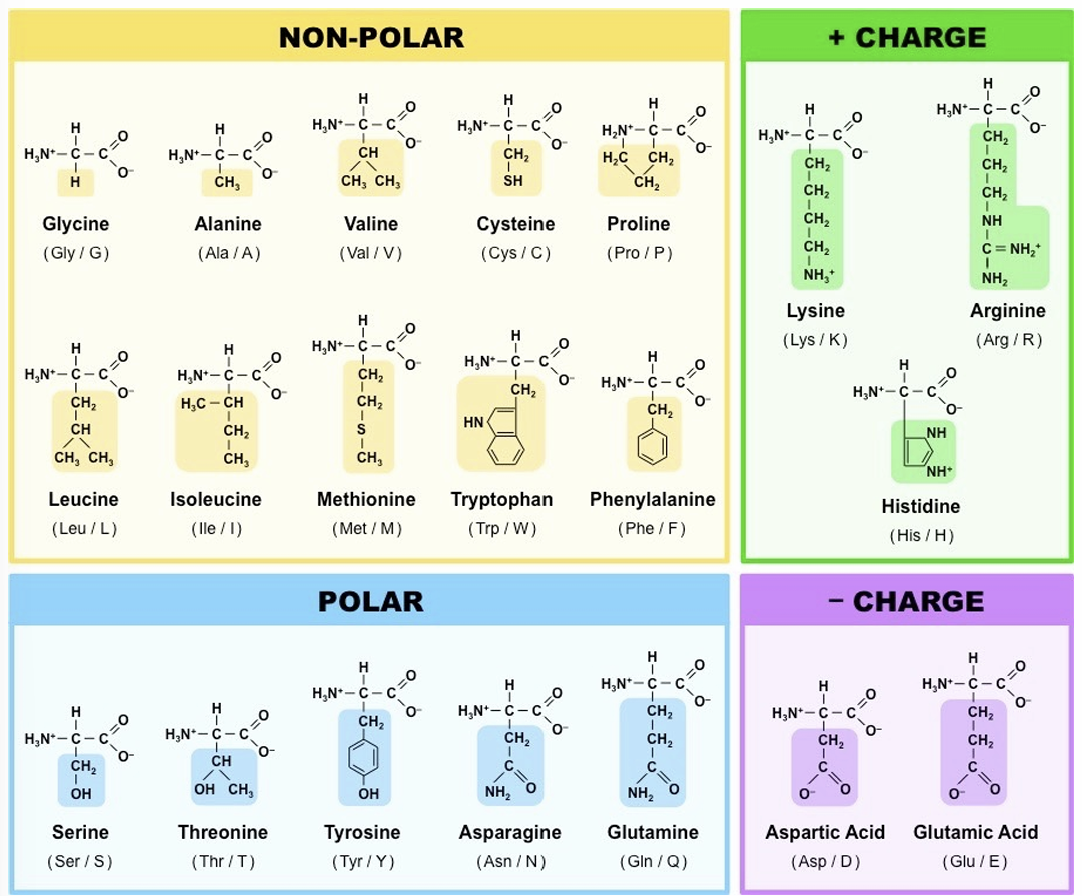
\includegraphics[width=\linewidth]{AA_structure.png}
    \caption{Amino acid structure}
    \label{fig:AA_struc}
\end{figure}

\subsubsection{amino acid hydrophobicity scores}




\begin{table}[H]
\centering
\rotatebox{90}{
\begin{tabular}{|l|c|c|c|c|c|}
\hline
\textbf{Amino Acid} & \textbf{3-Letter} & \textbf{1-Letter} & \textbf{Hydrophobicity / Hydropathy Index} & \textbf{Polarity} & \textbf{Acidity (pH)} \\
\hline
Alanine & Ala & A & 1.8 & Nonpolar & Neutral \\
Arginine & Arg & R & -4.5 & Polar & Basic (Strongly) \\
Asparagine & Asn & N & -3.5 & Polar & Neutral \\
Aspartate (Aspartic acid) & Asp & D & -3.5 & Polar & Acidic \\
Cysteine & Cys & C & 2.5 & Polar & Neutral \\
Glutamate (Glutamic acid) & Glu & E & -3.5 & Polar & Acidic \\
Glutamine & Gln & Q & -3.5 & Polar & Neutral \\
Glycine & Gly & G & -0.4 & Nonpolar & Neutral \\
Histidine & His & H & -3.2 & Polar & Basic (Weakly) \\
Isoleucine & Ile & I & 4.5 & Nonpolar & Neutral \\
Leucine & Leu & L & 3.8 & Nonpolar & Neutral \\
Lysine & Lys & K & -3.9 & Polar & Basic \\
Methionine & Met & M & 1.9 & Nonpolar & Neutral \\
Phenylalanine & Phe & F & 2.8 & Nonpolar & Neutral \\
Proline & Pro & P & -1.6 & Nonpolar & Neutral \\
Serine & Ser & S & -0.8 & Polar & Neutral \\
Threonine & Thr & T & -0.7 & Polar & Neutral \\
Tryptophan & Trp & W & -0.9 & Nonpolar & Neutral \\
Tyrosine & Tyr & Y & -1.3 & Polar & Neutral \\
Valine & Val & V & 4.2 & Nonpolar & Neutral \\
\hline
\end{tabular}
}
\caption{hydrophobicity scores Amino acids}
\label{tab:amino_acids_rotated}
\end{table}



\subsection{membrane embedding}
Membrane proteins can be 1 of many different forms but in general they can be divided into:\textbf{ Lipid anchors} or \textbf{transmembrane proteins}. membrane proteins face key challanges when folding compared to soluble proteins as they have to \textbf{expose hydrophobic residues} as opposed to the usual hydrophic collapse. This means they often need chaperone proteins to help them fold. (from bio last year fyi )


\subsubsection{transmembrane proteins}

\begin{figure}[H]
    \centering
    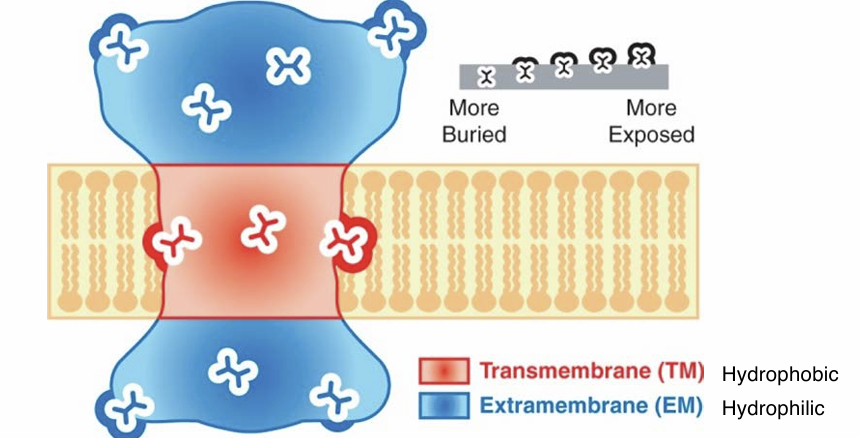
\includegraphics[width=0.5\linewidth]{MP_structure_overview.png}
    \caption{general structural requirements of a membrane protein}
    \label{fig:MP_struct_overview}
\end{figure}


transmembrane proteins need to be \textbf{\gls{amphiphilic}} in nature. This is needed as the membrane passing domain needs to be hydrophobic, however the domains not embeded in the membrane are exposed to water and need to be hydrophilic. Transmembrane protein will \textbf{contain either alpha helixes or beta sheets but not both} This mean we can divide them into to classes: transmembrane helix and beta barrels.
\begin{figure}[H]
    \centering
    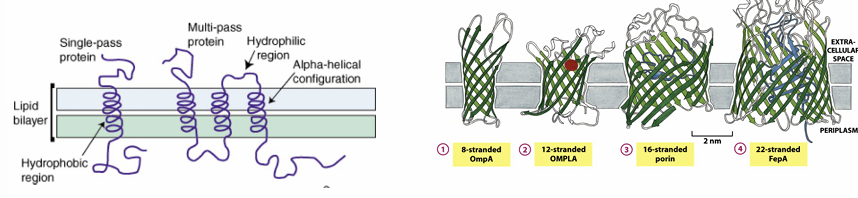
\includegraphics[width=\linewidth]{A_B.png}
    \caption{beta barrels vs transmembrane helix}
    \label{fig:enter-label}
\end{figure}

\paragraph{transmembrane helix}
Transmembrane helixes consist of alpha-helixes that have hydrophobic residues allowing them to pass through the membrane. An alpha helix has \textbf{3.6AA per turn} and each \textbf{turn is 5.4A long}. This means that a helix passing though the membrane which is around 3nm this will take 20 amino acids perpendicularly. However A helix does not have to cross perpendicularly so it's size can vary. Also note that  the \textbf{membrane thickness varies and these fluctuations may have a role in localization}.\textbf{ In general  membrane proteins are asymmetric}
 There are always exceptions:
 It is possible to have a charged a.i. in one transmembrane 
helix, forming for example an ionic interaction with another 
charged a.i. of another helix
\begin{figure}[H]
    \centering
    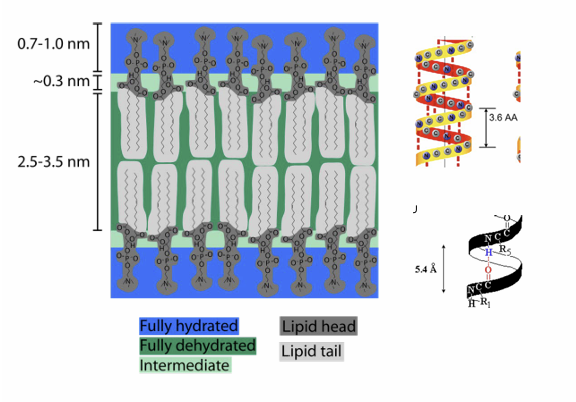
\includegraphics[width=0.5\linewidth]{helix_overview.png}
    \caption{helix stats}
    \label{fig:enter-label}
\end{figure}

\subparagraph{predicting transmembrane helices}
\begin{figure}[H]
    \centering
    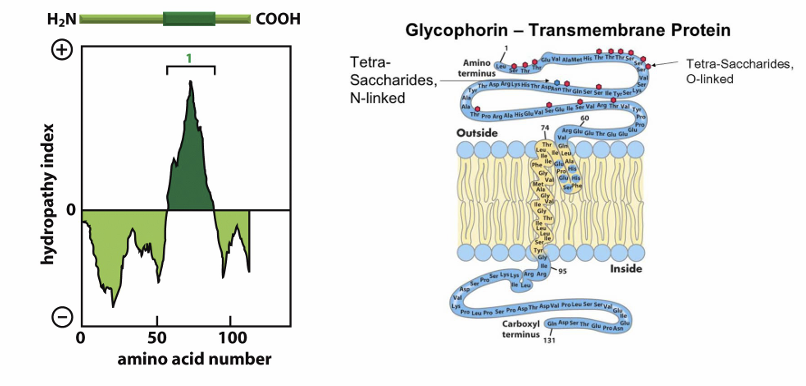
\includegraphics[width=0.5\linewidth]{transmembrane_helix.png}
    \caption{Predicting Transmembrane helices based on hyrophobicity score}
    \label{fig:enter-label}
\end{figure}
It is possible to predict transmembrane helices off of the \textbf{\gls{hydrophobicity_score}} which is an average of the $\pm$ 9 residues from the one being mesured. This is important as it gives an overall estiate of the local hydrophobicity of this part of the protein. the \textbf{window is chosen to be 19 as around 20AA is needed to cross the membrane}.

\paragraph{beta barrels}

\begin{figure}[H]
    \centering
    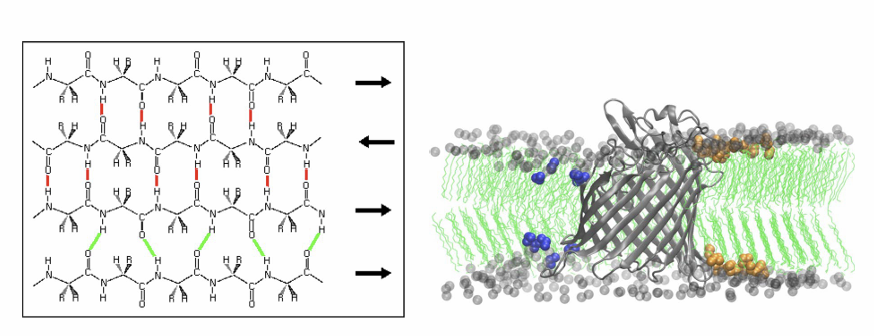
\includegraphics[width=0.5\linewidth]{Sum_Cell_Bio_II//lectures//cbII2/BBarrel.png}
    \caption{\gls{betaBarrel}}
    \label{fig:enter-label}
\end{figure}
Beta strands are quite different compared to transmembrane helices. Since beta strands have two sides. transmembrane proteins crosisting of beta strands take up a beta barrel shape. where one side of the strand has hydrophobic residues on the outisde while the otherside of the strand has hydrophilic residues. These then fold to form a barrel hence beta barrell.

\subparagraph{A cool side note: The membrane attack complex}

\begin{figure}[H]
    \centering
    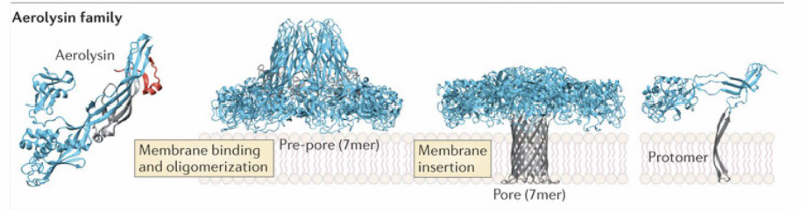
\includegraphics[width=0.5\linewidth]{MAC.png}
    \caption{membrane attack complex}
    \label{fig:enter-label}
\end{figure}

A rather cool protein of this group is the so called membrane attack complex which is giant protein that shoves it'self in the membrane and then assembles into beta barrel therby making a huge hole. This the kills the cell and is used among other things to kill bacteria and tumor cells.


\subsubsection{lipid anchors}
\begin{figure}[H]
    \centering
    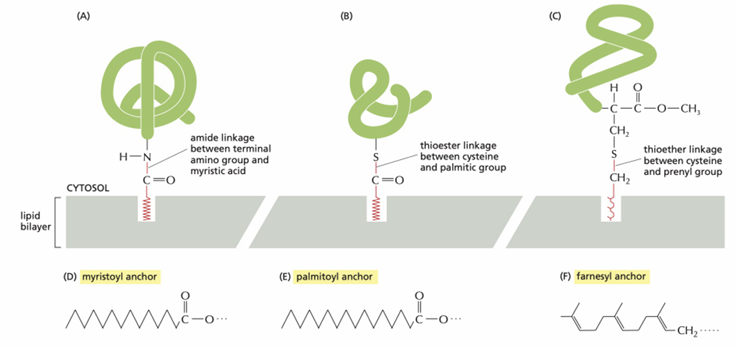
\includegraphics[width=0.5\linewidth]{Sum_Cell_Bio_II//lectures//cbII2/lipid_anchors.png}
    \caption{3 main types of lipid anchors}
    \label{fig:enter-label}
\end{figure}
Lipid anchors serve to hold part of a protein in place on the membrane. \textbf{Most of the time the anchor is on the inside of the cell} They are also important for membrane localization. There are 3 main types of lipid anchors:
\begin{itemize}
    \item myristol anchor
    \item palmitoyl anchor (this is the \textbf{only reversible lipidic modifition})
    \item farnesyl anchor
    
\end{itemize}

\paragraph{special case: GPI anchor}

\begin{figure}[H]
    \centering
    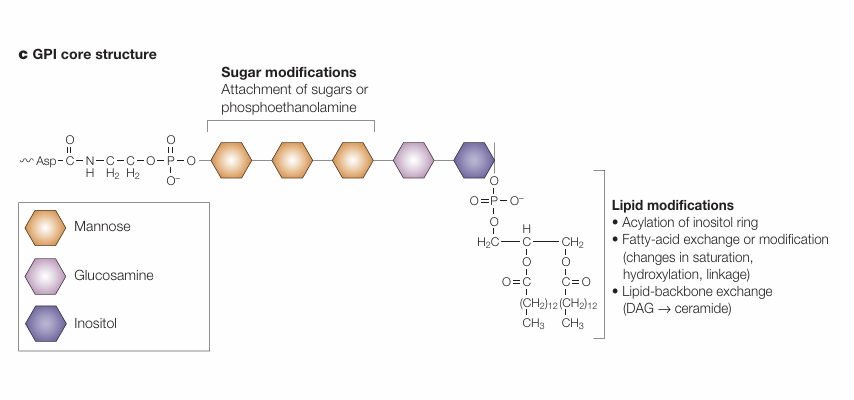
\includegraphics[width=\linewidth]{GPI.png}
    \caption{GPI anchor structure}
    \label{fig:enter-label}
\end{figure}
The GPI anchor is special as it is actually on the \textbf{outside of the cell} even though PI usually is on the cytosolic side! 

\subparagraph{the carbohydrate layer of the cell}

\begin{figure}[H]
    \centering
    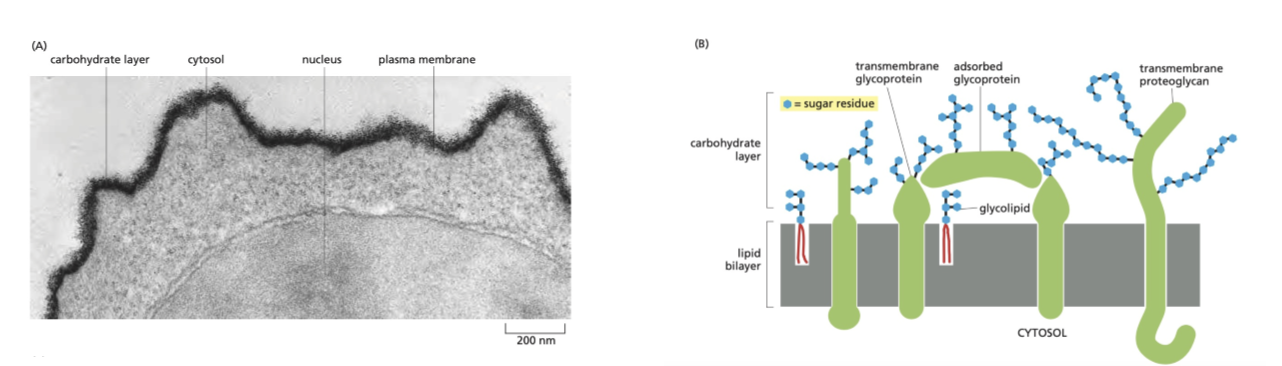
\includegraphics[width=0.5\linewidth]{Carbohydrate_layer.png}
    \caption{The carbohydrate layer of the cell membrae}
    \label{fig:enter-label}
\end{figure}

The cell membrane has a lot of glycolipids sticking out. (we will look at later I think..)


\subsection{membrane protein isolation}
\begin{figure}[H]
    \centering
    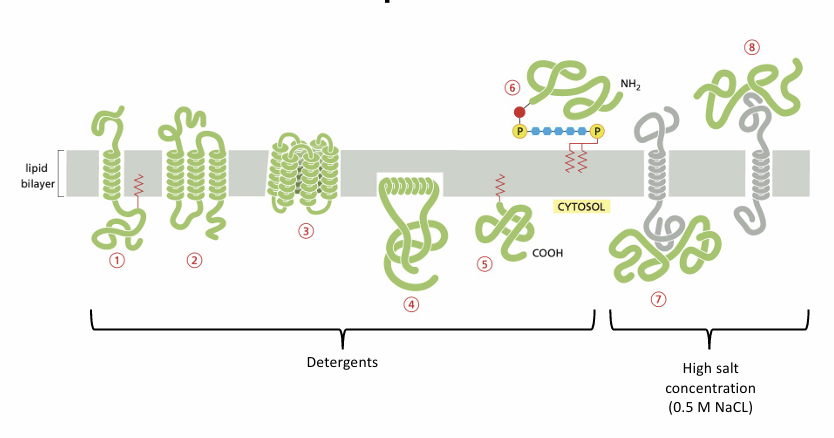
\includegraphics[width=0.5\linewidth]{MP_isolation.png}
    \caption{isolation of membrane proteins}
    \label{fig:enter-label}
\end{figure}
\textbf{The figure shows the following:}
\begin{enumerate}
    \item single pass alpha helix
    \item multipass alpha helix
    \item Beta-barrel
    \item alpha helix partitioned in the cytosolic monolayer of the lipid
    \item covalently linked to a lipid
    \item anchored to GPI on the outside
    \item non covalent binding to another protein
    \item non covalent binding to another protein
\end{enumerate}

In general detergents are needed to isolate membrane proteins but if they are non covalently bound to a protein in the membrane these can be detached with high salt concentrations.

\subsubsection{detergents}

\begin{figure}[H]
    \centering
    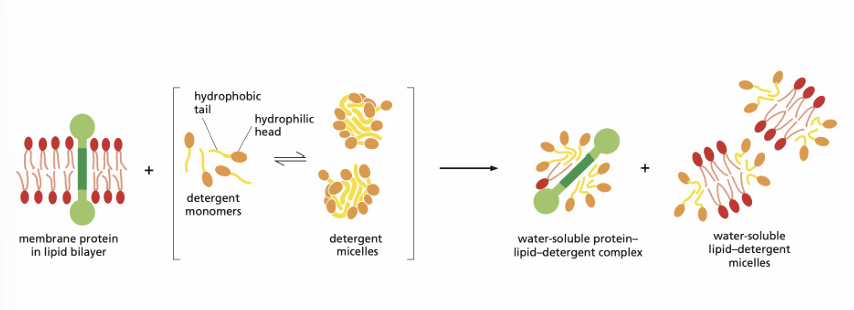
\includegraphics[width=\linewidth]{detergents.png}
    \caption{Detergents function}
    \label{fig:enter-label}
\end{figure}
Detergents are aphiphilic molecules that help solubilize membrane proteins. The ones seen in class are:
\begin{enumerate}
    \item \textbf{\gls{sds}} The negative charge will denature them though
    \item \textbf{\gls{tritonX100}} this detergent is less harsh than sds so will not denature the proteins. This is called \textbf{\gls{softSolubilization}} and is usefull when you want to isolate the protein in functional conformation.
    
\end{enumerate}


\subsubsection{nanodiscs}
\begin{figure}[H]
    \centering
    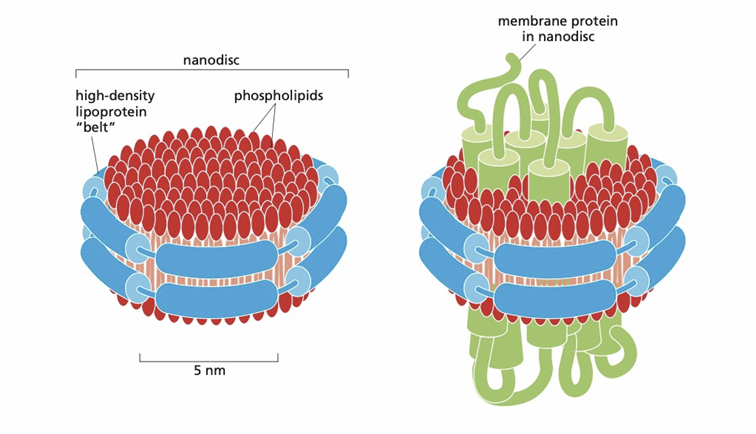
\includegraphics[width=0.5\linewidth]{nanodiscs.png}
    \caption{Nanodiscs}
    \label{fig:enter-label}
\end{figure}
Another cool method of isolating membrane proteins is to put them on so called \textbf{nanodiscs}. These are essentially tiny membrane pieces that are held together by a lipoprotein belt. 

\subsection{membrane protein localization}
\begin{figure}[H]
    \centering
    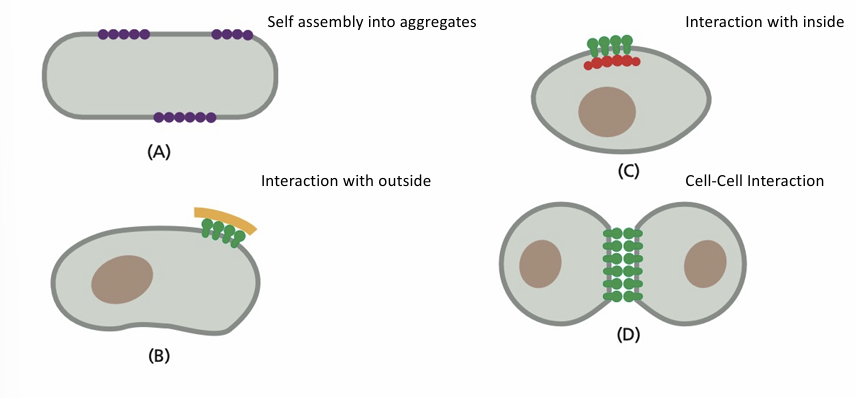
\includegraphics[width=0.5\linewidth]{localization.png}
    \caption{membrane protein localization mechanisms}
    \label{fig:enter-label}
\end{figure}

The cell membrane is very fluid and dynamic however membrane proteins need to be kept at certain places of the cell. This is essential for survival as the cell depends on having the right proteins at the right place. To do this it has 4 methods for restricting lateral mobility of specific membrane proteins:

\begin{enumerate}
    \item self assembly into aggregates. These can then form specific domains
    \item interation with outside 
    \item interactino with inside
    \item cell cell interactions
\end{enumerate}

The\textbf{ memrbane proteins can also affect how the membrane bends}

\begin{figure}[H]
    \centering
    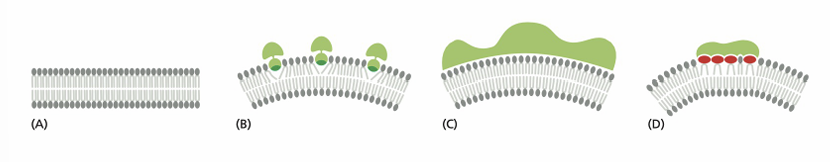
\includegraphics[width=\linewidth]{bending.png}
    \caption{membrane protein bending}
    \label{fig:enter-label}
\end{figure}
this can be acheived by  \textbf{(b)}wedging themselves in the membrane, \textbf{(c)}by physically pulling on the membrane, or \textbf{(d)} by binding to lipids with large head groups and stabilizing the curvature of the membrane 


\subsubsection{special case: Restriction by the cytoskeleton (spectrin- based)}

\begin{figure}[H]
    \centering
    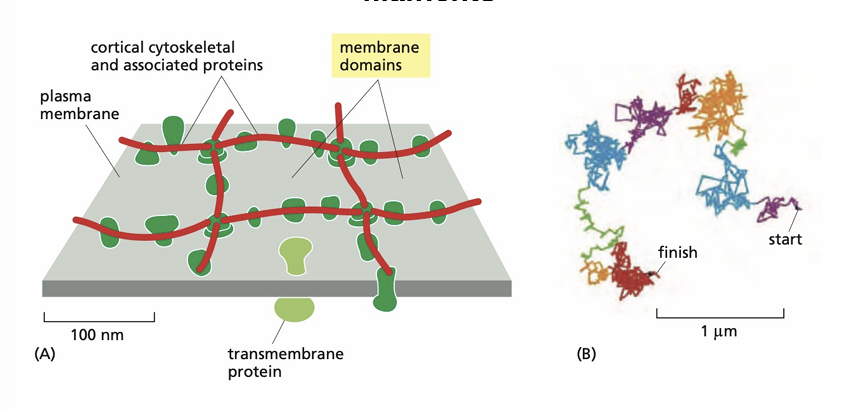
\includegraphics[width=\linewidth]{spectrin.png}
    \caption{\gls{spectrin} corraling plasma membranes}
    \label{fig:enter-label}
\end{figure}

A rather special case of membrane localization is that of\textbf{ spectrin} which is primarly found in red blood cells. This protein acts like a litteral fence therby corraling off certain domains on the plasma membrane and ensureing that the proteins inside stay in a certain area of the membrane. Kinda like sheep just chilling in a field.


\end{document}